% !Mode\dots ``TeX:UTF-8''
% !TEX root = ../bare_jrnl.tex


\section{Introduction}
\label{sec:intro}


\IEEEPARstart{I}n 1960s, Nobel Prize laureates Jacob and Monod~\cite{Jacob1961Genetic} found that ``Any cell contains a number of regulatory genes that act as switches and can turn one another on and off. If genes can turn one another on and off, then you can have genetic circuits.'' Inspired by these Boolean-type actions in genetic circuits, Boolean networks (\BNs) were firstly proposed by Kauffman \cite{Kauffman1968Metabolic} for modeling nonlinear and complex biological systems. 

{\BNs} are a type of discrete-time dynamical systems which can be represented as directed graphs. In a BN, each node has only two values ``0" and ``1", and they can change in different time points.  For a node $n_i$, we use $n_i(t)$ to denote its value at time $t$.
In general, $n_i(t+1)$ is determined by a logical function of $n_j(t),\ldots,n_p(t)$ if  there are  edges from $n_j,\ldots,n_p$ to $n_i$.  
%The logical operators used in  the logical functions include AND, OR, NO, XOR.  
Some general descriptions of the \BNs\ and their applications to biological systems can be found in~\cite{Kauffman1968Metabolic}. There exists a large number of  system works, both natural and artificial, which are modelled as \BNs, e.g. ~\cite{Akutsu2000Inferring, Shmulevich2002From, Faur2006Dynamical,Green2007The,Lou2010Multi}.
 \JP{Here, what do you mean by `systems works'?}

\BNs\ can be naturally extended to Boolean control networks (\BCNs) with external regulations and perturbations~\cite{Ideker2001A}. \BCNs\ have been applied to  various real-life problems. Cases of application can be found in 
structural and functional analysis of signaling and regulatory networks~\cite{Kaufman1999A, Klamt2006A}, 
abduction based drug target discovery~\cite{Biane2017Abduction}, 
and pursuing evasion problems in polygonal environments~\cite{Thunberg2011A}.
%
There are three kinds of nodes in \BCNs:  {\em input-nodes}, {\em state-nodes}  and {\em output-nodes}. At any moment of time each node takes a Boolean value.  The value of an output-node at time point $t$ (where $t\geq 0$)  depends on the values of state-nodes at time $t$, but the value of a  state-node at time point $t+1$  is determined by a  Boolean function of the values of the input-nodes and state-nodes at time point $t$. However,  we can only control the  values of the input-nodes and observe those of the output-nodes. Thus,  we cannot observe how   the values of the state-nodes change from time to time. Therefore, it is important to find a way to determine the initial values of the state-nodes at $0$ after observing a sequence of values of  input-nodes and their corresponding  values of the output-nodes. This is in general known as the {\em observability} of a \BCN.



Observability is one of the two basic  properties related to  the control-theoretic problems of \BCNs. The other is known as {\em controllability}. The work in ~\cite{Akutsu2007Control} shows that the problem of determining the controllability of \BCNs\ is {NP}-hard. Moreover, it  points out that ``One of the major goals of systems biology is to develop a control theory for complex biological systems.''  Since then, research on  controllability and observability of \BNs\ and \BCNs\ has drawn a great attention, e.g. \cite{cheng2009controllability, Zhao2010Input, Cheng2011Identification, Cheng2011Analysis} and \cite{Fornasini2013Observability}. %There, it is further noted that the controllability and observability are the basic control-theoretic problems of \BCNs. % Among these studies, \emph{semi-tensor product} (\STP) is one of useful tools to deal with  

 The concept of observability was first proposed in~\cite{cheng2009controllability}. It is mainly about how  to determine  the values of the  state-nodes  of a \BCN\  at time $0$ from the values of  input-nodes  and output-nodes at a sequence of time points $0,\ldots, k$. After that, four types of observability have been investigated in the literature,
 together with their corresponding determining algorithms, which we will discuss below.

\begin{figure}[!t]
      \centering
      \framebox{\parbox{3in}{
		\centerline{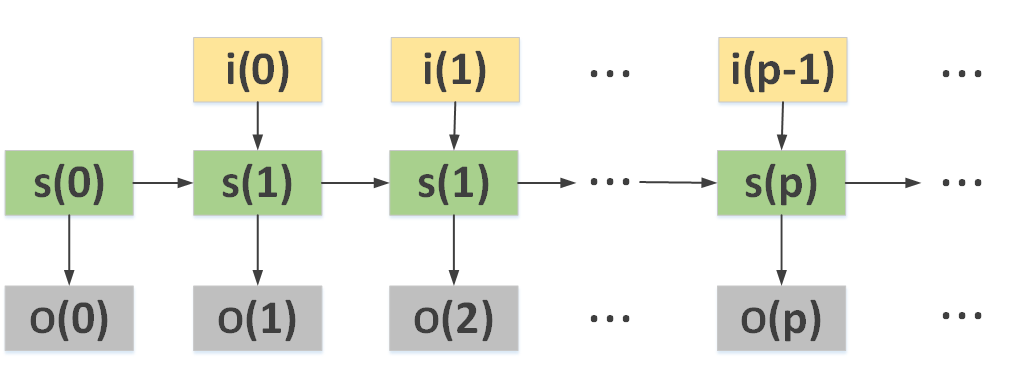
\includegraphics[scale=0.17]{figures/Fig10.png}}
	}}
      
      \caption{The relationship of inputs, states and outputs.}
      \label{fig:10}
  \end{figure}

Given a \BCN\ with $\ell$ input-nodes $(\mathsf{i}_1,\ldots, \mathsf{i}_\ell)$, $m$ state-nodes $(\mathsf{s}_1,\ldots, \mathsf{s}_m)$ and $n$ output notes  $(\mathsf{o}_1,\ldots, \mathsf{o}_n)$,  we use an {\em input vector} $\mathsf{i}(t)=(\mathsf{i}_1(t)\ldots\mathsf{i}_\ell (t))$, a {\em state vector} $\mathsf{s}(t)=(\mathsf{s}_1(t), \ldots \mathsf{s}_m(t))$ and an {\em output  vector} $\mathsf{o}(t)=(\mathsf{o}_1(t) \ldots \mathsf{o}_n(t))$  to represent an assignment of Boolean values to the  input-nodes, state-nodes and  output-nodes at $t$, respectively.  We call them an {\em input}, a {\em state} and an {\em output} of the \BCN\ at time time $t$. As  illusreated by Fig.~\ref{fig:10},  the state $\mathsf{s}(t+1)$ at time $t+1$ is determined by the input   $\mathsf{i}(t)$ and state $\mathsf{s}(t)$ at $t$  and the output   $\mathsf{o}(t)$ by the state  $\mathsf{s}(t)$.  We call a state $\mathsf{s}(0)$ at time $0$ an {\em initial state}. Thus, for any $k>0$ and any  initial state $\mathsf{s}(0)$, the states  $\mathsf{s}(1),\ldots, \mathsf{s}(k)$ and the output sequence $\mathsf{o}(1)\ldots, \mathsf{o}(k)$ are  determined by an  input sequence $\mathsf{i}(0),\ldots, \mathsf{i}(k-1)$.
%That is for a given  \BCN\  $\BB$,  $\mathsf{o}(0)\mathsf{o}(1)\ldots\mathsf{o}(k)$ is decide by $\mathsf{s}(0)$ and the sequence $\mathsf{i}(0)\mathsf{i}(1)\ldots\mathsf{i}(k-1)$. 
%
The four existing notions of observability of \BCNs\ can thus be described as follows. 
\begin{enumerate}
\item The  {\bf type-I}  observability was proposed in 2009 \cite{cheng2009controllability}. It states that a \BCN\ $\BB$ is observable if for any initial state   $\mathsf{s}(0)$ there exists an input sequence  $\mathsf{i}(0),\mathsf{i}(1),\ldots,\mathsf{i}(k-1)$ which can  distinguish $\mathsf{s}(0)$ from any other initial state $s'(0)$. That is,  given an initial state $\mathsf{s}(0)$, there is an input sequence $\mathsf{I}(k)=\mathsf{i}(0),\mathsf{i}(1),\ldots,\mathsf{i}(k-1)$ such that  for any  $\mathsf{s}'(0)$ which is different from $\mathsf{s}(0)$, the output sequence  $\mathsf{O}(k)=\mathsf{o}(0),\mathsf{o}(1),\ldots,\mathsf{o}(k)$ produced by  $\mathsf{s}(0)$ and $I(k)$ is different the output sequence  $\mathsf{O}'(k)=\mathsf{o}'(0),\mathsf{o}'(1),\ldots, \mathsf{o}'(k)$ produced by  $\mathsf{s}'(0)$ and $\mathsf{I}(k)$.

\item The  {\bf type-II} observability was proposed in 2010 \cite{Zhao2010Input}. It states that a \BCN\ $\BB$ is observable if for every two different initial states $\mathsf{s}(0)$ and $\mathsf{s}'(0)$, there exists an input \JP{`inout'? or `input'?} sequence $\mathsf{i}(0),\mathsf{i}(1),\ldots, \mathsf{i}(k-1)$ that can distinguish $\mathsf{s}(0)$ and $\mathsf{s}'(0)$. More precisely speaking,  for any pair of different initial  $\mathsf{s}(0)$ and $\mathsf{s}'(0)$, \JP{Why use $\mathsf{s}^{y}(0)$?}
there exists an input sequence  $\mathsf{i}(0),\mathsf{i}(1),\ldots,\mathsf{i}(k-1)$ such that the output sequences $\mathsf{o}(0),\mathsf{o}(1),\ldots,\mathsf{o}(k)$ and  $\mathsf{o}'(0),\mathsf{o}'(1),\ldots,\mathsf{o}'(k)$ corresponding to  the different initial states  $\mathsf{s}(0)$ and $\mathsf{s}'(0)$, respectively, are different.
	
\item The  {\bf type-III} observability was proposed in 2011 \cite{Cheng2011Identification}.  It states that a \BCN\ $\BB$ is observable if for any $k>0$ there is a sequence $\mathsf{i}(0),\mathsf{i}(1),\ldots, \mathsf{i}(k-1)$ that distinguishes every pair of different initial states. This means that in $\BB$, there exists an input \JP{`inout'?} sequence  $\mathsf{i}(0),\mathsf{i}(1), \ldots,\mathsf{i}(k-1)$ such that for any two different initial states $\mathsf{s}(0)$ and $\mathsf{s}'(0)$, the output sequence $\mathsf{o}(0),\mathsf{o}(1), \ldots, \mathsf{o}(k)$  corresponding to  $\mathsf{s}(0)$  is different from the output sequence  $\mathsf{o}'(0),\mathsf{o}'(1),\ldots, \mathsf{o}'(k)$ corresponding to $\mathsf{s}'(0)$.
\JP{Please don't change notations. Stick to $s(0)$ and $s'(0)$. $\mathsf{s}^{x}(0)$ and $\mathsf{s}^{y}(0)$ are somehow strange.}
	
\item  The  {\bf type-IV}  observability was  proposed in 2013 \cite{Fornasini2013Observability}. It states that a \BCN\ $\BB$ is observable if every sufficient long $\mathsf{i}(0)$$\mathsf{i}(1)\ldots$$\mathsf{i}(k-1)$ genertaes different output sequences  from different initial states. Precisely speaking, there is a big enough number $M$, for every  input sequence $\mathsf{i}(0),\mathsf{i}(1),\ldots, \mathsf{i}(k-1)$ which is not shorter than $M$, the output sequences $\mathsf{o}(0), \mathsf{o}(1), \ldots, \mathsf{o}(k)$ and  $\mathsf{o}'(0), \mathsf{o}'(1), \ldots, \mathsf{o}'(k)$ produced by the inout sequence from every two different initial states $\mathsf{s}(0)$ and $\mathsf{s}'(0)$, respectively, are different.
\end{enumerate}
 We will give the formal definitions of these four types of observability and discussion their relations in Section~\ref{sec:pre}.
 \JP{So far, I don't see a clear difference among the first three types from the above description.}

%\JP{Here, you need an introductory sentence on why algorithms are needed.}
%Four types of observability develop different algorithms to determine $\mathsf{s}(0)$ of \BCN. 
Let $\mathsf{S}(t)$ denote the set of possible valuations of $\mathsf{s}(t)$.

For the {\bf type-I} observability, if a \BCN\ is observable then we can determine its $\mathsf{s}(0)$ by following procedure. 
\begin{description}
	\item[Step 1] We infer $\mathsf{S}(0)$ by the $\mathsf{o}(0)$ based on the relation of $\mathsf{o}(t)$ and $\mathsf{s}(t)$. Then for every $\mathsf{s}'(0)\in\mathsf{S}(0)$, it has a corresponding $\mathsf{i}(0),\mathsf{i}(1),\ldots,\mathsf{i}(k-1)$.
	\item[Step 2] We choose a $\mathsf{s}'(0)$ from $\mathsf{S}(0)$, and input its corresponding $\mathsf{i}(0),\mathsf{i}(1),\ldots,\mathsf{i}(k-1)$. If $\mathsf{s}(0)=\mathsf{s}'(0)$ we can determine $\mathsf{s}(0)$ from the output sequence of \BCN, else we reset the state of \BCN\ by $\mathsf{s}(0)$. We repeat Step 2 until we can determine $\mathsf{s}(0)$.
	
\end{description}

 For the {\bf type-II} observability, if a \BCN\ is observable then we can determine its $\mathsf{s}(0)$ by following procedure. 
\begin{description}
	\item[Step 1] We infer $\mathsf{S}(0)$ by the $\mathsf{o}(0)$ based on the relation of $\mathsf{o}(t)$ and $\mathsf{s}(0)$. 
	\item[Step 2] We input a $\mathsf{i}(0),\mathsf{i}(1),\ldots,\mathsf{i}(k-1)$ which can help us further determine $\mathsf{S}(0)$ from the output sequence of \BCN. We repeat step 2 until $|\mathsf{S}(0)|=1$, such that we can determine $\mathsf{s}(0)$.
\end{description}

 For the {\bf type-III} observability, if a \BCN\ is observable then we can determine its $\mathsf{s}(0)$ by inputing the $\mathsf{i}(0),\mathsf{i}(1),\ldots,\mathsf{i}(k-1)$ that distinguish every pair of different initial states and observing the output sequence of \BCN.

For the {\bf type-IV} observability, if a \BCN\ is observable then we can determine its $\mathsf{s}(0)$ by inputing any sufficient long $\mathsf{i}(0),\mathsf{i}(1),\ldots,\mathsf{i}(k-1)$ and observing the output sequence of \BCN.
%{\color{red} (13)}

Loosely speaking, different ways to determine $\mathsf{s}(0)$ are proposed for different applications, and the four types of observability present whether the \BCNs\ can be determine by these four ways respectively. Both {\bf type-I} and {\bf type-II} determine $\mathsf{s}(0)$ by repeating the process of inputing $\mathsf{i}(0),\mathsf{i}(1),\ldots,\mathsf{i}(k-1)$. While {\bf type-III} and {\bf type-IV} determine $\mathsf{s}(0)$ by taking this process once, because in some applications we cannot repeat this process. %And the second observability is the necessary and sufficient condition of determining $\mathsf{s}(0)$ by taking the determining procedure once. 
\JP{What applications?}

In this paper, we address the necessary and sufficient condition of determining $\mathsf{s}(0)$ by taking the determining process once to make \BCN\ be able to apply to more applications.
\JP{Here, `necessary and sufficient condition' appears for the first time. What are their precise definitions?}
Naturally there is a procedure to determine $\mathsf{s}(0)$  which is described as follows.
\JP{Why in this way it can be applied to more applications?}
%It enriches the control-theory of \BCNs, it can help us determine the $\mathsf{s}(0)$ of some \BCNs\ which can not be determined before.

%\begin{problem}
%\label{pro:1}
%For a given \BCN\ $\BB$, whether its initial state $\mathsf{s}(0)$ can be determined by carrying on determining procedure once?
%\end{problem}

%Although, these four existing notions of observability can help us study some information about $\mathsf{s}(0)$ we need. 
%The problem means that whether the $\mathsf{s}(0)$ can be determined if the determining procedure can do at most once. %only third and fourth ones  can  determine the $\mathsf{s}(0)$ of \BCNs.
%Only third and fourth notions of observability can help us solve the {\em Problem~\ref{pro:1}}.
% What is more, in the third observability, a \BCN\ is observable iff there is an input sequence that determines its initial state $\mathsf{s}(0)$. Thus its condition is very strong, and the condition of fourth observability is even stronger.
%However, 
%Let $\mathsf{S}(t)$ denote the set of possible valuations of $\mathsf{s}(t)$. Then naturally there is a procedure which is described as follows.
%We find that to determine $\mathsf{s}(0)$ by taking the determining procedure once we only need to complete the following procedure. 

%Informly, the procedure of our  online observability as follows. 
 %Then $\mathsf{S}(t)$ can be derived by the output sequence $\mathsf{o}(0)\mathsf{o}(1)\ldots\mathsf{o}(t)$, input sequence $\mathsf{i}(0)\mathsf{i}(1)\ldots\mathsf{i}(t-1)$ and updating rules of $\BB$.
 
 %\tl{can you make this a proper algorithm?}\gs{I have corrected this one.}
\begin{description}
	\item[Step 1] We infer $\mathsf{S}(t)$ by the $\mathsf{o}(t)$ based on the relation of $\mathsf{o}(t)$ and $\mathsf{s}(t)$.
	\item[Step 2] According to the relation of $\mathsf{i}(t)$, $\mathsf{s}(t)$ and $\mathsf{s}(t+1)$ we choose an $\mathsf{i}(t)$ which would not make every two distinct $\mathsf{s}^{x}(t)$ , $\mathsf{s}^{y}(t)$$\in$ $\mathsf{S}(t)$ become the same state after affected by $\mathsf{i}(t)$ i.e. $\mathsf{s}^{x}(t+1)\ne\mathsf{s}^{y}(t+1)$. Such that, for every $\mathsf{s}^{x}(t+1)\in $ $\mathsf{S}(t+1)$ there is exact one corresponding $\mathsf{s}^{x}(t)\in $ $\mathsf{S}(t)$.
	\item[Step 3] Repeating Step 1 and Step 2 we can determine $\mathsf{s}(t)$, and for every $t>0$, for every $\mathsf{s}^{x}(t)\in \mathsf{S}(t)$ there is exact one corresponding $\mathsf{s}^{x}(t-1)\in \mathsf{S}(t-1)$, so we can determine $\mathsf{s}(t-1)$, \ldots, $\mathsf{s}(0)$.
\end{description}

%In the third observability, we can finish this procedure, thus we can determine the initial state \State$(0)$ for a \BCN. What is more, 


%Such that, the requirement for a \BCN\ to determine \State$(0)$ would be easist to satisfy. 
%{\color{red} (13)} 
Inspired by this procedure, we propose a new notion of observability named online observability to address the necessary and sufficient condition of determining $\mathsf{s}(0)$ by taking the determining procedure once. It states that a \BCN\ $\BB$ is observable if the previously mentioned procedure would terminates for every \State$(0)$. Its formal definitions will be presented in Section~\ref{sec:online}. 

We call this observability online observability, because we observe $\mathsf{o}(t)$ of \BCN\ and choose $\mathsf{i}(t)$ based on the information we have collected so far at every time $t$. 
\JP{It is very unclear why we need this new notion and why it is supposed to be better.}
\JP{In general, the introduction lacks of a good motivation for the current research.
Can you somehow re-structure the introduction?
1. What is the context of this paper?
2. What exactly is the research problem and why it is important?
3. What are the existing solutions and why they are not sufficient?
4. What is your new solution and its main idea?
5. Why is your new solution better?
6. Any evidence to support your claim?}

In contrast, in the {\bf type-III} and {\bf type-IV} observability we determine $\mathsf{s}(0)$ of \BCN\ by its recorded $\mathsf{o}(0)\mathsf{o}(1)\ldots\mathsf{o}(k)$ after we input $\mathsf{i}(0)\mathsf{i}(1)\ldots\mathsf{i}(k-1)$, and  we do not interfere with \BCN\ except for the logging of its inputs and outputs, thus we call them offline observability \cite{Cassar2017A}. %{\color{red} (13)}

%Then, in this paper we make the following contributions. 
\medskip\noindent
{\bf Contributions.}
Firstly, we propose and formally define the online observability. % to address the necessary and sufficient condition of determining $\mathsf{s}(0)$ by taking the determining procedure once. %It enriches the control-theory of \BCNs. 
Secondly, we also provide a determination algorithm for the online observability. Finally, we present some optimization brought by the online observability. Including the means to find shortest path and the approach to avoid entering critical states in the process of determining the initial states of \BCNs.  These optimization further explain the advantages of online observability of \BCNs. 

\medskip\noindent
{\bf Plan of the paper.}
The remainder of this paper is organized as follows.
 {\em Section \ref{sec:pre}} introduces necessary preliminaries about \BCNs, including the definition of \BCNs\ and four existing observability. {\em Section \ref{sec:online}} presents the definition of online observability of \BCNs. {\em Section \ref{sec:deter}} presents the determination algorithm for online observability. 
% {\em Section \ref{sec:app}} talks about some optimization brought by the online observability of \BCNs. 
 {\em Section \ref{sec:con}} ends up with the introduction of our future work.

%==============================================================================================================